\section{LTC n-dimension compare with Regression}

From the previous experiments, we know that LTC has good performance on 
data sets \english{which has long constant and same differences}. \english{If high-order
regression method would work better in real activity data sets \TG{This isn't a correct
English sentence \ldots}}. In this
paragraph, we compare Polynomial Regression \TG{refer to description in ch2} with LTC in different dimensions. 

% need  a graph for polynomial regression with different p,  by using 200Hz
% walking and running data set, also need a table to show the RMSE and
% compression ratio, Max error.

\subsection{Implementation of Polynomial Regression}

We implemented polynomial regression method to compress 3D acceleration data
($t$, $a.x$, $a.y$, $a.z$). In the data-set, we process polynomial regression
with the relationship between independent variables $t$ (Time-stamp) and dependent
variables $a.x$, $a.y$ and $a.z$. For tolerance checking, we use infinity norm
and Euclidean norm. The implementation needs much memory to record data points,
and some CPU time to compute coefficients. \TG{Link to your implementation?}
\TG{You didn't explain in Ch2 how polynomial regression was extended to dim n.}

\begin{figure}
  \centering
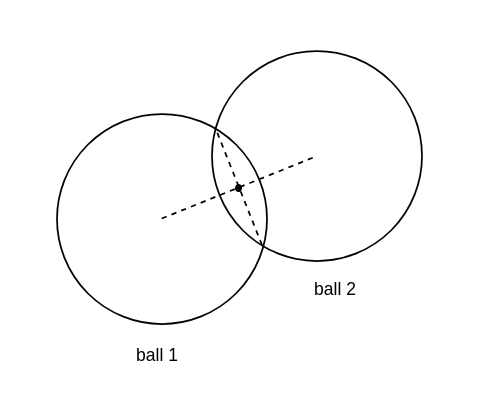
\includegraphics[width=0.7\textwidth]{figures/point-in-chord.png}
\caption{The point selected to determine the direction}
\label{fig:compare_point}
\end{figure}
\TG{Figure 7 shows in the next chapter, you should fix that.  }

We use Polynomial Regression method on previous walking and running data set.
Figure~\ref{fig:poly-regression} shows the result. \TG{Wrong reference, there isn't
a Figure 8d.}

\begin{figure*}
\centering
\begin{subfigure}{\columnwidth}
\centering
\includegraphics[width=0.3\columnwidth]{figures/regression-p3-in-x.pdf}
\includegraphics[width=0.3\columnwidth]{figures/regression-p3-in-y.pdf}
\includegraphics[width=0.3\columnwidth]{figures/regression-p3-in-z.pdf}
\caption{Regression degree=3 with Infinity norm}
\end{subfigure}
{\footnotesize}

\centering
\begin{subfigure}{\columnwidth}
\centering
\includegraphics[width=0.3\columnwidth]{figures/regression-p3-Eu-x.pdf}
\includegraphics[width=0.3\columnwidth]{figures/regression-p3-Eu-y.pdf}
\includegraphics[width=0.3\columnwidth]{figures/regression-p3-Eu-z.pdf}
\caption{Regression degree=3 with Euclidean norm}
\end{subfigure}

\centering
\begin{subfigure}{\columnwidth}
\centering
\includegraphics[width=0.3\columnwidth]{figures/regression-p5-in-x.pdf}
\includegraphics[width=0.3\columnwidth]{figures/regression-p5-in-y.pdf}
\includegraphics[width=0.3\columnwidth]{figures/regression-p5-in-z.pdf}
\caption{Regression degree=5 with Infinity norm}
\end{subfigure}
{\footnotesize}

\centering
\begin{subfigure}{\columnwidth}
\centering
\includegraphics[width=0.3\columnwidth]{figures/regression-p5-Eu-x.pdf}
\includegraphics[width=0.3\columnwidth]{figures/regression-p5-Eu-y.pdf}
\includegraphics[width=0.3\columnwidth]{figures/regression-p5-Eu-z.pdf}
\caption{Regression degree=5 with Euclidean norm}
\label{fig:poly-regression}
\end{subfigure}

\end{figure*}

\subsection{Results of Comparison}
In our implementation, for a regression model which has N-degree and
M-parameters we need M*(N+1) coefficients and extra time-stamp used to record
where should the model stop. In the Table , It obvious that LTC n-dimension work
better than Polynomial regression, because it need more bytes to save the
coefficients. In our case, coefficients are recorded as float points which would
use 4 bytes per each. The total number of bytes needed to represent original
data is (N+1)*M*4+4 (Int32 for Time-stamp). Polynomial regression using more
processing time to calculate coefficients and build model when each new data
point comes.
\begin{table}[]
\begin{tabular}{|l|l|l|l|l|l|l|l|}
\hline
           & \multicolumn{2}{c|}{LTC} & \multicolumn{2}{c|}{Regression degree = 3} & \multicolumn{3}{l|}{Regression degree = 5}\\ \hline
Dimension & Infinity   & Euclidean   & Infinity    & Euclidean     & Infinity      & \multicolumn{2}{l|}{Euclidean} \\ \hline
1          & 90.1\%     & 90.1\%      & 89\%        & 89\%          & 88.96\%       & \multicolumn{2}{l|}{88.96\%}   \\ \hline
2          & 89.6\%     & 88.7\%      & 83.35\%     & 83.35\%       & 83.55\%       & \multicolumn{2}{l|}{83.1\%}    \\ \hline
3          & 88.9\%     & 87.6\%      & 80.24\%     & 78.68\%       & 80.8\%        & \multicolumn{2}{l|}{77.96\%}   \\ \hline
\end{tabular}
\caption{Walking \TG{What are the \% here? Compression ratio?} \TG{This table and the next one are not referenced or discussed in the text!}}
\end{table}


\begin{table}[]
\begin{tabular}{|l|l|l|l|l|l|l|l|}
\hline
           & \multicolumn{2}{c|}{LTC} & \multicolumn{2}{c|}{Regression degree = 3} & \multicolumn{3}{l|}{Regression degree = 5}          \\ \hline
Dimension & Infinity   & Euclidean   & Infinity            & Euclidean           & Infinity& \multicolumn{2}{l|}{Euclidean} \\ \hline
1          & 74.7\%     & 74.7\%      & 70.7\%      & 70.7\%        & 71.1\%        & \multicolumn{2}{l|}{71.1\%}    \\ \hline
2          & 70.6\%     & 68.6\%      & 58.3\%      & 57.4\%        & 58.4\%        & \multicolumn{2}{l|}{57.35\%}   \\ \hline
3          & 68.6\%     & 64.4\%      & 51.1\%      & 48\%          & 50.2\%        & \multicolumn{2}{l|}{47.92\%}   \\ \hline
\end{tabular}
\caption{Running}
\end{table}
